% ======================= Pre-Amble =========================

\documentclass[11pt, oneside]{article}   	% use "amsart" instead of "article" for AMSLaTeX format 
                     						%imports package {article} and specify option(s) [11pt, oneside]
\usepackage{geometry}                		% See geometry.pdf to learn the layout options. There are lots.                                        

\geometry{letterpaper}                   		% ... or a4paper or a5paper or ... 
%\geometry{landscape}                		% Activate for rotated page geometry

\usepackage[parfill]{parskip}    		        % Activate to begin paragraphs with an empty line rather than an indent

\usepackage[hidelinks]{hyperref}                % Allows for clickable references

%American Mathematics Society packages
\usepackage{amsmath}	   %math
\usepackage{amssymb}       %symbols
\usepackage{amsthm}          %theorems

%Graphics
\usepackage{graphicx}
\usepackage[usenames, dvipsnames]{color}     % font colour:    \textcolor{<colour>}{text}
      									%highlight text:  \colorbox{<color>}{text}
									
									%list of colours: https://www.sharelatex.com/learn/Using_colours_in_LaTeX

%Images		                
\graphicspath{ {images/} }                          %directory that your images are located in within your current directory
	

%Footnote Spacing
\setlength{\footnotesep}{0.4cm}                  %specify spacing b/w footnotes
\setlength{\skip\footins}{0.6cm}                    % space b/w footnotes and textbody

%Table
\usepackage[none]{hyphenat}                    % Stops breaking-up words in a table (i.e. no hyphens)
                                                               

\usepackage{array}   
\newcolumntype{x}[1]{>{\centering\let\newline\\\arraybackslash\hspace{0pt}}p{#1}}       %center fixed column width: x{<len>}                      
\newcolumntype{$}{>{\global\let\currentrowstyle\relax}}                                                   % let us apply things (e.g. bold/italicize) to entire row            
\newcolumntype{^}{>{\currentrowstyle}}
\newcommand{\rowstyle}[1]{\gdef\currentrowstyle{#1} #1\ignorespaces}

%Bibliography
\usepackage[numbers,sort&compress]{natbib}   %for multiple references: sorts  (i.e. [1,2] NOT [2, 1] )
                                           				  %                                     compresses (i.e. [1-3] )
\usepackage[nottoc]{tocbibind}                            %add bibliography to table of contents

%Diagrams
\usepackage[latin1]{inputenc}
\usepackage{tikz}
\usetikzlibrary{shapes,arrows}
	

\usepackage{dirtytalk}    %quotations: use \say  

\usepackage{caption}
\captionsetup[figure]{labelfont=bf}    %make figure labels boldface
\captionsetup[table]{labelfont=bf}     %make table labels boldface

% ======================== Document ======================
\begin{document}

\title{Local Search Algorithm for University Class Schedule Optimization \\
\line(1,0){360} \\               %(slope x, y){length of line}
\vspace{1cm}
\large
The University of British Columbia \\
MATH 441 \\
November 27, 2015
\vspace{1cm}}


\author{
Knill, Stephanie\\
54882113
\and
Valdivieso, Mauricio\\
25216145
\and
Zhu, Ian\\
46888129
}

\date{}                    % Activate:  display a given date (e.g. {August 4} ) or no date (empty {} )
                                    %No activate: display current date
\maketitle

%\begin{abstract}
%Following the classification system employed by Peng et al. (2009), courting behaviour will be recorded if either panda (1) approaches a sexual partner forwardly, presenting estrous or rutting behaviors, such as shaking head, urinating/defecating, rubbing gentile, etc.; (2) bleats ''Mie, Mie'', stares at the partner, sniffs the partner's urine, feces, or the leftover scent mark; or (3) scratches the partner in order to attract his or her attention. Additionally, a successful copulation will be recorded if the male panda's penis penetrates the female panda's vagina and at a latter time a high chirp cry from the female is heard; a failed copulation will be recorded if the keeper has to separate the two pandas because they bit or attacked each other, seldom approached each other in the pen, or display waning courtship. 
%\end{abstract}

\thispagestyle{empty}    %do not display page number on this page


% ================= Table Of Contents ================
\cleardoublepage
\tableofcontents

\thispagestyle{empty}   %do not display page number on this page




% ================= Background/Relevance ================

\cleardoublepage
\setcounter{page}{1}    %set page number to 1 (b/c want to start on first page of contents)

\section{Background}

While the University of British Columbia (UBC) is committed to \say{[providing] support and programming initiatives designed to remove barriers for students with disabilities and facilitate disability related accommodations for members of the UBC Vancouver community} \cite{ref:access}, the onus is still upon the students to optimize their time at University, given their own unique and diverse set of constraints. In late August of the year 2015, a member of our group befell a most grievous injury that relegated her to the mercy of crutches. Weeks later when the subsequent winter term started, she was unable to attend her classes---those she did attend she was thoroughly late for\footnote{A conspiracy theory of her trying to trip a mathematics professor in an attempt to \say{crutch him up} was also in rampant circulation.} and was only pardoned from the walk-of-shame that befalls all latecomers due to her pitiable state---owing to the expansive, sprawling nature of the UBC Vancouver campus. Deeply concerned for our comrade's well-being, we wanted to do something to alleviate her plight. What if this had been more than a temporary state? How would she be able to finish her degree whilst still maintaining a competitive enough grade point average (GPA) to fulfill her childhood dreams of mathematics graduate school? So we took her course schedule and minimized the walking distance between classes.

Or in Ian's words, we optimized laziness.

\subsection{University Class Schedule}
As a second year undergraduate majoring in mathematics at UBC, there are a number of required (critical) courses for her to be eligible for promotion to third year (MATH 200, 215, 220, 221 and CPSC 210\footnote{MATH 210 or CPSC 210 may be taken to fulfill the mathematical computing requirement. We would like to take more computer science courses in upper years, however, so we will be taking CPSC 210 instead.}), as well as 15 credits (5 courses) of electives. Additionally, many of these courses have pre-requisite and co-requisite requirements: 
\begin{itemize}
\item MATH 215, 340: requires MATH 221
\item MATH 300, 302, 317: requires MATH 200
\item MATH 215: co-requires MATH 200
\item MATH 300: co-requires MATH 317
\end{itemize}

Thus, MATH 200 and 221 must be taken in the first term while MATH 215 must be taken in the second term. If either MATH 300, 302, 317, 340 are taken as electives, they will be taken in term two. Using the data provided on the UBC Student Service Centre (SSC) for the 2015-2016 Winter Session, a table of the class locations, time, and term(s) offered for all sections of the critical classes (Table~\ref{critical}) and desired electives (Table~\ref{elective}) was constructed.

\begin{table}[h]                                          %optional argument: place figure/table here (h), top (t), page of floats (p)
\begin{center}
\begin{tabular}{$p{0.8 in} | ^p{0.7in}^p{0.6in}^p{0.7in}^p{0.9in}^c^c }  
    \multicolumn{7}{c}{\textbf{Critical Classes}} \\
    [0.5cm]              %row skip \\[<len>], where <len> is any length
    \rowstyle{\bfseries} & Building & Room & Days & Time & Section & Term  \\          
    \hline  				
    MATH 200 & LSK & 201 & MWF & 9:00 - 10:00 & 101 & 1 \\
     & LSK & 201 & MWF & 11:00 - 12:00 & 102 & 1 \\
     & ANNEX & 1100 & MWF & 11:00 - 12:00 & 103 & 1 \\
     & BUCH A  & 104 & MWF & 13:00 - 14:00 & 104 & 1 \\
     & BUCH A & 201 & TTh & 9:30 - 11:00 & 105 & 1 \\
     & BUCH A & 104 & TTh  & 15:30 - 17:00 & 107 & 1 \\
     [0.1cm]
    \hline
    MATH 221 & LSK & 201 & MWF & 10:00 - 11:00 & 102 & 1 \\
     & MATH & 100 & MWF & 13:00 - 14:00 & 103 & 1 \\
     & LSK & 201 & MWF & 13:00 - 14:00 & 104 & 1 \\
     [0.1cm]
    \hline
    MATH 220 & ANNEX & 1100 & MWF & 12:00 - 13:00 & 101 & 1 \\
     & LSK & 200 & MWF & 10:00 - 11:00 & 102 & 1 \\
     & LSK & 460 & MWF & 10:00 - 11:00 & 103 & 1 \\
     [0.1cm]
    \hline
    MATH 215 & ANNEX & 1100 & MWF & 10:00 - 11:00 & 201 & 2 \\
    & BUCH A & 201 & MWF & 9:00 - 10:00 & 202 & 2 \\
    [0.1cm]
    \hline
    CPSC 210 & WOOD & 101 & MWF & 12:00 - 13:00 & 101 & 1 \\
     & HUGH & 310 & MWF & 14:00 - 15:00 & 102 & 1 \\					

\end{tabular}
\end{center}
\caption{Table of class locations, time, term(s) offered for all sections of critical classes.}
\label{critical}
\end{table}



\begin{table}[h]                                          %optional argument: place figure/table here (h), top (t), page of floats (p)
\begin{center}
\begin{tabular}{$p{0.85 in} | ^p{0.7in}^p{0.6in}^p{0.7in}^p{0.9in}^c^c }  							
    \multicolumn{7}{c}{\textbf{Elective Classes}} \\
    [0.5cm]
    %\multicolumn{7}{c}{} \\
    \rowstyle{\bfseries} & Building & Room & Days & Time & Section & Term  \\          
    \hline     
    MATH 300 & ANNEX & 1100 & TTh & 14:00 - 15:30 & 201 & 2 \\
     & ANNEX & 1100 & MWF & 13:00 - 14:00 & 202 & 2 \\
     [0.1cm]
    \hline	
    MATH 302 & LSK & 201 & MWF & 11:00 - 12:00 & 201 & 2 \\
    [0.1cm]
    \hline		
    MATH 317 & LSK & 460 & MWF & 14:00 - 15:00 & 201 & 2 \\
     & BUCH A & 202 & MWF & 12:00 - 13:00 & 202 & 2 \\
     [0.1cm]
    \hline
    MATH 340 & MATH & 104 & TTh & 9:30 - 11:00 & 201 & 2 \\
    & BUCH A & 103 & MWF & 12:00 - 13:00 & 202 & 2 \\
    [0.1cm]
    \hline
    BIOL 317 & MCML & 160 & MWF & 9:00 - 10:00 & 101 & 1 \\
    %BIOL 343 & BIOL & 2200 & MWF & 14:00 - 15:00 & 101 & 1 \\
    %PHIL 321A & CHEM & D200 & MWF & 9:30 - 11:00 & 001 & 1 \\

\end{tabular}
\end{center}
\caption{Table of class locations, time, term(s) offered for all sections of elective classes.}
\label{elective}
\end{table}

Although on paper math majors experience a relatively large amount of freedom in choosing electives and math courses to fulfill graduation requirements, the competitiveness of graduate school and the prospective job market add further constraints. In an effort to maximize GPA, Calculus IV (MATH 317) will be taken in the second term in the hopes of still remembering materials from Calculus III (MATH 200) in first term. Calculating one's probability of getting into graduate school has also been deemed an asset---Introduction to Probability (MATH 302) is a much needed wake-up call. Likewise, it has been rumoured that the MATH 441 professor has nice math shirts; the pre-requisite Introduction to Linear Programming (MATH 340) must also be taken. Due to a childhood rumination with plant taxonomy, Weed Science (BIOL 317) is also essential. 

Given these constraints for graduation requirements (required courses, credit requirements, pre-requisites \& co-requisites), personal preferences, and different sections offered, our goal is to write a program that yields a class schedule that minimizes walking distance.

\subsection{The Local Search Algorithm}

Rather than utilizing an exhaustive search method, the local search algorithm was favoured due to its relative computational efficiency. The local search algorithm attempts to find the optimal solution to a given optimization problem through many small, local changes. Initially given a feasible solution, each successive iteration makes a local or relatively simple change to the current solution, thereby creating another feasible solution. This cycle continues until either a time bound (i.e. number of iterations) has been met or when a solution is considered optimal (i.e. the best obtainable solution in the neighbourhood cannot be improved).

In the procedure known as \say{hill-climbing}, the local search algorithm picks the best neighbouring solution or any solution that is an improvement of the current solution. Although this method guarantees that each new solution is at least as good as the previous solution, one may arrive at a local optimal solution---not the global optimal solution. Our algorithm addresses this problem. Specifically, our code \say{randomly} produces a nearby feasible schedule and sets this as the current schedule. Thus, we are not bound to any local path and the entire search space may be explored with enough iterations.

% ================= Methodology ================
\cleardoublepage
\section{Methodology}

\subsection{Calculating Walking Distance}
In order to calculate the distance between any two locations on campus, a cartesian coordinate system in $\mathbb{R}^2$ was mapped onto the UBC Vancouver campus (Figure~\ref{grids}). Utilizing the Global Positioning System (GPS) provided by Google Maps, each square has side length of 50 metres.

\begin{figure}[h]                                   
\begin{center}
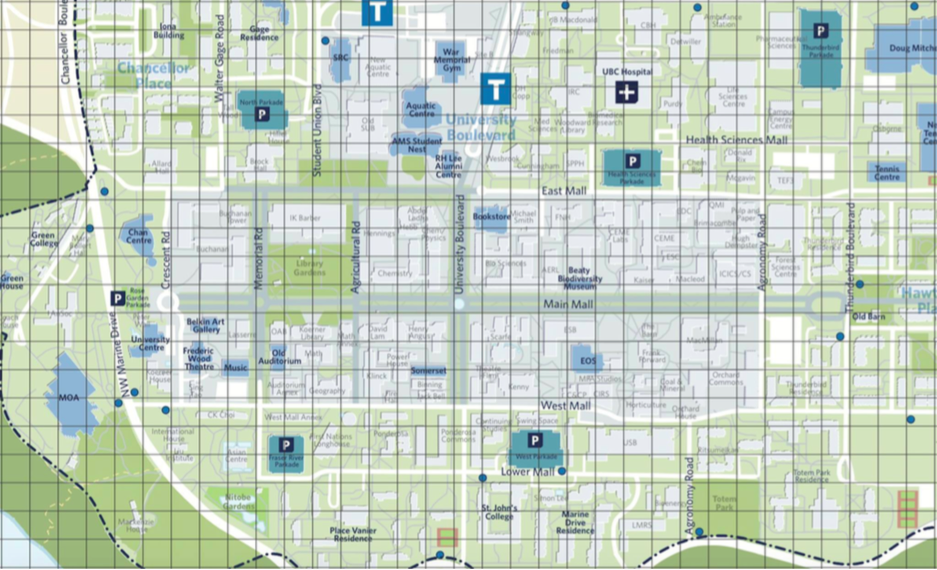
\includegraphics[width=.9\textwidth]{grids.jpg}
\caption{Cartesian coordinate map of the University of Building Construction (UBC), with origin set as bottom left coordinate. Each unit increment is 50m.}
\label{grids}
\end{center}
\end{figure}

Using this we were able to generate a unique $(x,y)$ coordinate for each classroom building and the  bus loop (Table~\ref{building}). Due to the excessive presence of blue fences on campus, the $L^1$-norm was favoured over the Euclidean-norm in calculating the distance between classes. On a more serious note, crutches' lack of mobility (inability to cut corners, traverse grass), the grid-like nature of UBC pathways, and the modern day infeasibility of walking diagonally through building walls were also weighty factors in this decision.


\begin{table}[h]                                          %optional argument: place figure/table here (h), top (t), page of floats (p)
\begin{center}
%\begin{tabular}{$c |^ c ^ c || ^c | ^c  ^c}  	
\begin{tabular}{$p{0.7 in} | ^c^p{0.2 in} || ^p{0.7in} |^c^c}  							
    \rowstyle{\bfseries} Building & x & y  & Building & x & y\\[0.1cm]          
    \hline        
    ANNEX & 12 & 8 & IKB & 11 & 12 \\
    BUCH A & 8 & 11 & LSK & 13 & 12 \\
    BIOL & 17 & 11 & MATH & 11 & 8 \\
    CHEM & 14 & 10 & MCML & 20 & 12\\
    HUGH & 26 & 12 & WOOD & 20 & 16\\
    ICICS & 26 & 10 & Bus Loop & 13 & 19\\

\end{tabular}
\end{center}
\caption{$(x,y)$ coordinate for buildings on UBC Vancouver campus.}
\label{building}
\end{table}

\newpage

\subsection{Our Local Search Algorithm}

Our local search works by taking an initial feasible schedule (consisting of classes $C_1, C_2, \ldots , C_{10}$) and performing the following procedure for a specified number of iterations. A single iteration can be broken down into three steps (Figure~\ref{method}):

\begin{enumerate}

\item A class $C_i$ is randomly selected and removed from the feasible schedule
\item Amongst a subset of the bank (consisting of all periods for $C_i$), a period of $C_i$ is randomly chosen to be placed back into the schedule. The period chosen may or may not be the same period of $C_i$ that was removed from the initial feasible schedule.

\item Insert class $C_i$ back into the schedule

\textit{\textbf{Case 1}: the resulting schedule is feasible.} Since the schedule is feasible, the iteration is complete. The next iteration will use this resulting feasible schedule as its initial feasible schedule.

\textit{\textbf{Case 2}: the resulting schedule is infeasible (the incoming $C_i$ is in a time slot of an already existing period in the schedule)} The incoming period $C_i$ replaces the conflicting class in the existing schedule. Since the schedule is still infeasible---we are missing one class---we return to step two. Now the subset of the bank refers to the class that was just replaced. This process will continue until a feasible schedule is reached (case 1), thus terminating the iteration\footnote{It is worth remarking that since we begin with a feasible schedule, every iteration will result in a feasible schedule---either the original feasible schedule or a new feasible schedule. In the unlikely case where there is only one feasible schedule, the iteration will always complete because it can return to its initial state; this still counts as a full iteration.}.
\end{enumerate}

\begin{figure}[h]

% Define block styles
\tikzstyle{decision} = [diamond, draw, fill=blue!20, 
    text width=4.5em, text badly centered, node distance=3cm, inner sep=0pt]
\tikzstyle{block} = [rectangle, draw, fill=blue!20, 
    text width=5em, text centered, rounded corners, minimum height=4em]
\tikzstyle{line} = [draw, -latex']
\tikzstyle{cloud} = [draw, ellipse,fill=red!20, node distance=3cm,
    minimum height=2em, text width=5em, text centered]
    
\begin{tikzpicture}[node distance = 3cm, auto]      %default setting of node distance =3cm
    % Place nodes: \node [block style] {reference} {Text displayed};
    \node [cloud] (init) {Feasible Schedule};                                                           
    \node [block, right of=init, node distance=3.25cm] (step1) {\textbf{Step 1}};     %increase node distance (OW nodes overlap)
    \node [block, right of=step1] (step2) {\textbf{Step 2}};
    \node [decision, right of=step2] (step3) {\textbf{Step 3}: feasible schedule?};
    \node [block, right of=step3, node distance=3.5cm] (case1) {\textbf{Case 1}};
    \node [block, below of=step3] (case2) {\textbf{Case 2}};
    
    % Draw edges: \path [edge style] (node1) -- (node2);
    \path [line] (init) -- (step1);
    \path [line] (step1) -- (step2);
    \path [line] (step2) -- (step3);
    \path [line] (step3) -- node  [near start] {yes} (case1);    %place text {yes} near the start of  node1
    \path [line] (step3) -- node [near start] {no}(case2);
    \path [line] (case2) -| (step2);              % |: arrow bends (horizontal -, then veritval | ??)
    \path [line,dashed] (case1) (12.75, 0.8) -- (12.75, 2) -- (0, 2) -- (0, 0.7) (init);     %arrow bends a lot so i specified coordinate locations of arrows
\end{tikzpicture}

\caption{Flow chart illustrating algorithm of our local search function. Dotted arrow (not step in iteration) indicates that each iteration terminates with a feasible schedule.}
\label{method}
\end{figure}

Under the assumption that the student begins and ends his or her day at the Bus Loop, the objective function value at each iteration is then computed using the $L^1$-norm. By computing the walking distance after each iteration, we can determine if the new solution represents an improvement over the previous best-found solution (the initial feasible schedule being the initial value to be improved upon). Since improvements are only stored, it becomes apparent that the last solution added to this list of solutions is the optimum solution.


Our (Java) code is divided amongst four main categories, known as packages (see Appendix A for full code):

%Appendix~\ref{AppendixA}

\begin{enumerate}
\item \textbf{Model}: contains all the code necessary to solve the problem. This package includes our representation of Buildings, Periods, Schedules, the Solver, and the final output. This package will be analyzed in more detail after we discuss the remaining packages.


\item \textbf{Parsers}: contains the code critical to read the raw data used by the \say{Model} package. Class schedule data for the 2015-2016 winter session from the UBC SSC was transcribed into an Excel Spreadsheet; although this format makes inputting easy and intuitive for most users running this local search function, Java is not such person. Using an online data convertor \cite{ref:convert}, the raw data (buildings, periods, and critical class data) was converted into JSON format, which Java can easily interact with through our coded parsers.  Due to the inefficiency of writing data directly into JSON format, this conversion method was favoured.

\item \textbf{Tests}: checks whether our code is behaving accordingly in each step, as well as the larger functions. This ensures every step is working as intended---we're not just getting a lucky answer that looks correct. 

\item \textbf{Tfl}: contains a bridge between the parsers and the raw data. The code in this package feeds the JSON data into the parsers to enable us to utilize our functions. All code from this package was taken from the CPSC 210 2015 Project Mind the Gap Phase 1. Although this package is essential to our application, it is in no particular way related to our algorithm for local search.
\end{enumerate}

Returning to the aforementioned \say{Model} package, there are several aspects of our code worth discussing to elucidate the inner workings of our algorithm and the project as a whole. A \textbf{Period} is defined by a class name, an $x$ and $y$ coordinate, a specific time, and a room number. The set of all periods is henceforth referred to as the \textbf{bank}. A \textbf{feasible schedule} is a subset of the bank that has every critical class exactly once and has no time conflicts (i.e. no two classes are taken at the same time). \textbf{Time Slots} are defined as a positive integer corresponding to a particular time period when a class at UBC takes place (Table~\ref{timeslot}). Our \textbf{Schedule Problem} is thus made up of the bank, a feasible schedule and a list of the names of critical subjects. 

\begin{table}[h]                                          %optional argument: place figure/table here (h), top (t), page of floats (p)
\begin{center}
\begin{tabular}{$p{1.2cm} | ^ x{2.9cm} || ^c |^c}                     %use x{<len>} to centre a column of length <len> 				
    \rowstyle{\bfseries} & Time Period & Time Slot (T1) & Time Slot (T2) \\[0.1cm]          
    \hline        
    MWF & 8:00-9:00 & 1 & 17 \\
    & 9:00-10:00 & 2 & 18 \\
    & 10:00-11:00 & 3 & 19 \\
    & 11:00-12:00 & 4 & 20 \\
    & 12:00-13:00 & 5 & 21 \\
    & 13:00-14:00 & 6 & 22 \\
    & 14:00-15:00 & 7 & 23 \\
    & 15:00-16:00 & 8 & 24 \\
    & 16:00-17:00 & 9 & 25 \\
    & 17:00-18:00 & 10 & 26 \\
    [0.1cm]
    \hline
    TTh & 8:00-9:30 & 11 & 27 \\
    & 9:30-11:00 & 12 & 28 \\
    & 11:00-12:30 & 13 & 29 \\
    & 12:30-14:00 & 14 & 30 \\
    & 14:00-15:30 & 15 & 31 \\
    & 15:30-17:00 & 16 & 32 \\
\end{tabular}
\end{center}
\caption{Time Slots and their corresponding time periods for classes at UBC Vancouver in Term 1 (T1) and Term 2 (T2).}
\label{timeslot}
\end{table}


After completing the designated number of iterations, the optimal solution is outputted to the user. This solution consists of Periods, whose data type is composed of an $x$ and $y$ coordinate, a room number, and a time slot. With this information, the building where the class takes place is tracked down through the Parsers. The output to the user only conveys the essential information, namely the walking distances of the list of improved solutions and the optimal class schedule. Deeply concerned with the user's potential mental breakdown when presented with ominous lines of code, we further simplified our output by omitting any terms or days that did not have classes scheduled. If you are not taking classes on Tuesdays and Thursdays for example, these days would be omitted in the final output. Specification of the number of iterations and the raw data of the desired classes are all that is required for our program to output an optimal class schedule. Armed with this sense of bliss and utmost serenity, the user may now press the mythically proportional run button. 


% ================= Results ================
\cleardoublepage
\section{Results}

Running our local search function in Java (Figure~\ref{fig:optimal})

\begin{figure}[h]                                   
\begin{center}
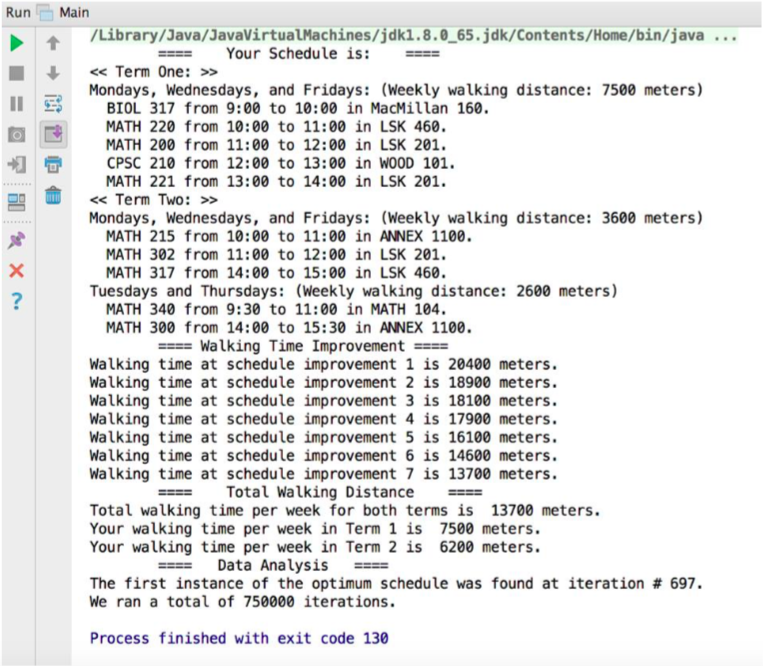
\includegraphics[width=.86\textwidth]{optimal.jpg}
\caption{\label{fig:optimal}Java output for optimal class schedule. Objective function is 13,700 meters.}
\end{center}
\end{figure}

yields an optimal solution of 13,700 meters, which was found on iteration 697 of 750,000\footnote{Each time the algorithm is run, the first instance of the optimal solution may be found on a different iteration.}. No classes in term 1 were scheduled on Tuesdays and Thursdays. To put this in more \textcolor{red}{c}\textcolor{Orange}{o}\textcolor{yellow}{l}\textcolor{green}{o}\textcolor{blue}{u}\textcolor{ProcessBlue}{r}\textcolor{Plum}{f}\textcolor{magenta}{u}\textcolor{Brown}{l} terms, our beloved crutched team member excitedly created a worklist of her new and improved class schedule using the UBC SSC course scheduling (Figure~\ref{fig:term2}).


\begin{figure}[h!]                                  
\begin{center}
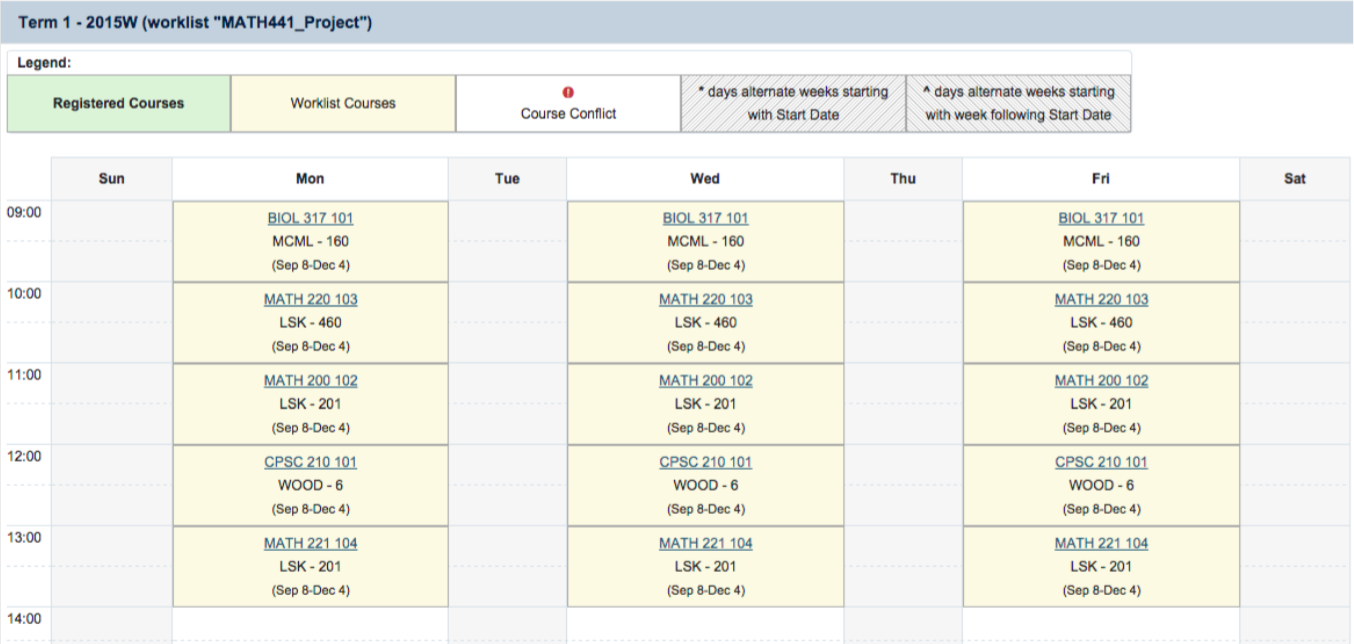
\includegraphics[width=.99\textwidth]{term1.png}
%\caption{\label{fig:term1}Optimal class schedule for term 1.}
\end{center}
\end{figure}

\begin{figure}[h!]    %! forces it to be here                                
\begin{center}
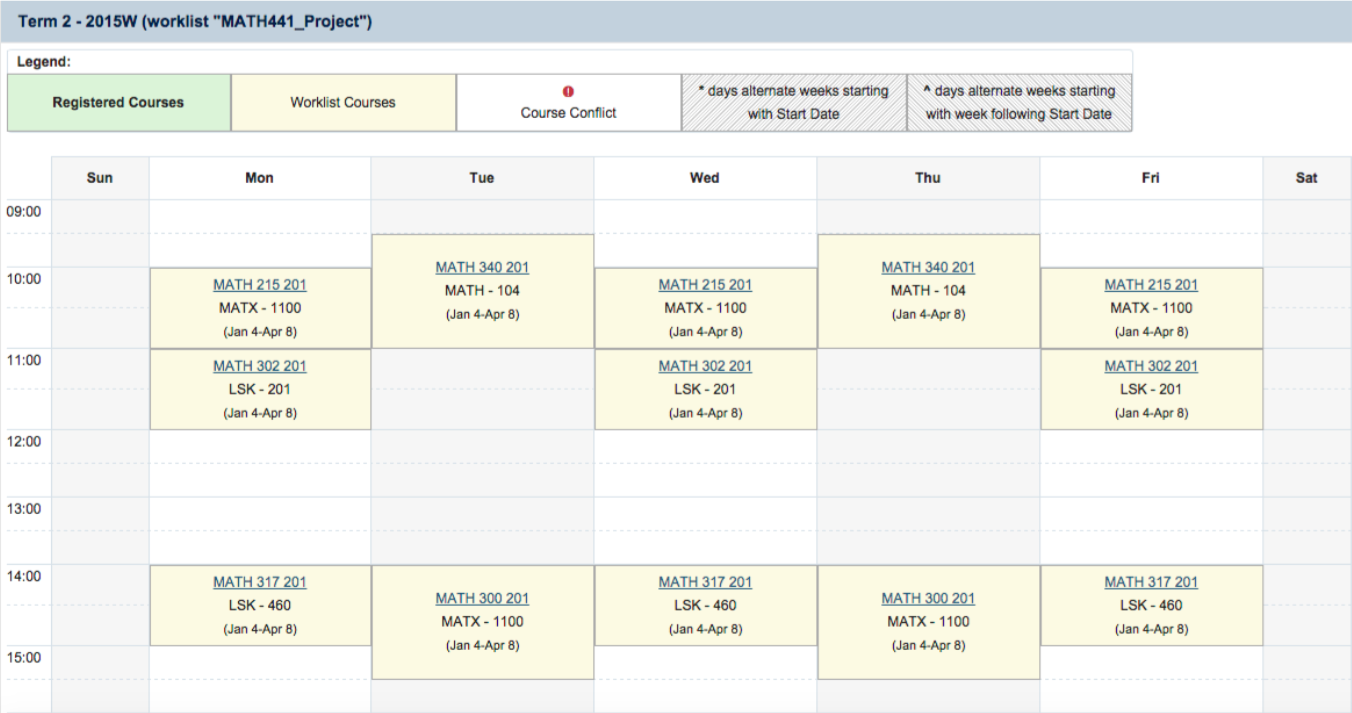
\includegraphics[width=.99\textwidth]{term2.png}
\caption{\label{fig:term2}Optimal class schedule for term 1 and 2.}
\end{center}
\end{figure}


% ================= Discussion ================

\cleardoublepage
\section{Discussion}


Looking at our raw data, there are 6 sections of MATH 200, 3 sections of MATH 221, 3 sections of MATH 220, 2 sections of CPSC 210, and 1 section of our most beloved Weed Science (BIOL 317) in Term 1. This corresponds to \textbf{108} possible permutations. In Term 2, we have 2 sections of MATH 215, 2 sections of MATH 300, 1 section of MATH 302, 2 sections of MATH 317, 2 sections of MATH 340. This corresponds to \textbf{16} possible permutations.

Since each permutation in Term 1 can correspond with any permutation from Term 2, we have a total of \textbf{1,728} permutations. However, many permutations will not be feasible schedules---a feasible schedule must consist of classes that are not defined on the same period. Thus, the set of feasible schedules is a much smaller subset of the list of total permutations. Running our random schedule generator (the one used to generate our initial feasible schedule) exhaustively yields a total of \textbf{640} different feasible schedules. 

\subsection{Efficiency of Local Search Algorithm}

Computationally, our local search on average finds the optimal feasible schedule after 1,000 trials.  Whereas some may decide at this point to go in guns-a-blazing, arguing passionately for a more efficient exhaustive search method, one might want to hear us out before embarking on this rampant escalation. 

While the project was still in its cradle stages, we identified a problem for our precious newborn: if we were to program our algorithm based off a greedy search, there would be a high probability of becoming stuck in a local solution. We also acknowledged, however, that a greedy search is highly efficient at producing near optimum solutions. But we wanted the best for our child---only the global optimum would do.\footnote{Looking back now, a decent near-optimal solution may have for all intents and purposes be optimal. A pity the 15-year race lecture came too late.} So we addressed this potentially devastating ailment by programming a random, rather than hill-climbing, local search algorithm. This allowed for bad moves in order to cover the entire search space, thus eventually generating the global solution.\footnote{In retrospect, it would have been interesting to write out a greedy approach and compare this with our current algorithm. However, experience has told us that not sleeping---while questionably feasible---is most definitely not optimal. Needless to say this proposed route of analysis was swiftly vetoed by the IT department.} Unfortunately, the results of our well-intentioned guidance resulted in an algorithm that was reminiscent of a less efficient exhaustive search method. Although both methods cover the entire sample space, our algorithm differs by also returning to previous solutions due to its random nature. 

\subsection{Sensitivity Analysis}

Since there are many ways to measure the sensitivity of our algorithm, we decided to examine the most practical case: the effect of blocking a certain period (i.e. you cannot schedule any classes during a certain time period) on the objective function. That is, we examined how the minimum travel distance is affected when certain time periods are booked for various activities, such as math TA duties, club meetings, lunch, sanity breaks, or an aversion to 8 am classes. If the removal of a time period results in an infeasible schedule, then it cannot be blocked off. For example, Weed Science only has 1 section (Time Slot 1), so this time period cannot be removed.

\subsubsection*{Assumptions}

Although we are blocking off a period for a specific purpose, we do not take into account the walking distance to the activity. While this may be the case if we book off a morning\footnote{Or afternoon} period to sleep-in, blocking off a class period to walk to the cafeteria for food does not increase the objective function. Had the location of the activity been taken into account, the true optimal schedule would most likely be different from our algorithm's outputted schedule. 

Although it would be relatively simple to block off two or more periods at a time (in terms of programming, the only alterations to the code are done by deleting the classes specified at a certain time period), we did not include this in our analysis as the possible permutations would get quite out of hand.

\subsubsection*{Results and Analysis}

The results of this analysis is summarized in Table~\ref{sensitivity}. The largest increase in the objective function is when Time Slot 4 (MWF 11:00-12:00) is blocked. 

\begin{table}[h]                                          %optional argument: place figure/table here (h), top (t), page of floats (p)
\begin{center}
\begin{tabular}{$l  ^c ^c ^ l}            %{$p{1.2cm} | ^ x{2.9cm} || ^c |^c}                     %use x{<len>} to centre a column of length <len> 


    \rowstyle{\bfseries} & Optimal Value & \% Difference & Affected Classes \\[0.1cm] 
    \hline
    \textbf{Term 1}\\					%\multicolumn{4}{l}{\textbf{Term 1}} \\
    \hline
    MWF 11:00-12:00 & 16100 & \textbf{17.518} & MATH 200 - 3 left (BUCH)\\[0.1cm] 
    MWF 12:00-13:00 & 14300 & 4.38 & MATH 220 - 2 left (LSK)\\
    &&& CPSC 210 - 1 left (HUGH)\\[0.1cm] 
    MWF 13:00-14:00 & 14300 & 4.38 & MATH 200 - 5 left\\
    &&&  MATH 221 - 1 left (LSK)\\[0.1cm] 
    MWF 14:00-15:00 & 13700 & 0 & CPSC 210 - 1 left (WOOD)\\[0.2cm] 
    \hline
    \textbf{Term 2 }\\ 
    \hline
    MWF 9:00-10:00 & 13700 & 0 & MATH 215 - 1 left (LSK) \\[0.1cm] 
    MWF 10:00-11:00 & 14000 & 2.19 & MATH 215 - 1 left (BUCH) \\[0.1cm] 
    MWF 12:00-13:00 & 13700 & 0 & MATH 317 - 1 left (MATH)\\
    &&& MATH 340 - 1 left (MATH) \\[0.1cm] 
    MWF 13:00-14:00 & 13700 & 0 & MATH 300 - 1 left (ANNEX) \\[0.1cm] 
    MWF 14:00-15:00 & 15500 & 13.139 & MATH 317 - 1 left (BUCH) \\[0.1cm] 
    TTh 9:30-11:00 & 13800 & 0.73 & MATH 340 -  1 left (BUCH) \\[0.1cm] 
    TTh 14:00-15:30 & 13800 & 0.73 & MATH 300 -  1 left (ANNEX) \\[0.1cm] 

\end{tabular}
\end{center}
\caption{Sensitivity Analysis when a certain time slot is blocked. Percentage Difference defined as $\frac{\text{New Value } - \text{ Optimal}}{\text{Optimal}}\cdot100\%$. Affected Classes indicates the classes where a section(s) is removed and the remaining number of sections with their respective locations.}
\label{sensitivity}
\end{table}


In general, the optimal travel distance is not extensively altered from single period blocks. This is due to second year math courses having many sections. Similarly, most math classes are offered in the region known as the Math Triangle (Math, Math Annex, LSK)---a region where a number of math professors and students have disappeared under mysterious circumstances. Thus, removing a single period generally has minimal effect on the overall walking distance, with the notable exception being Time Slot 4. Blocking off this time slot eliminates two sections of MATH 200 in LSK; the only remaining sections are in Buchanan\footnote{There is a fourth remaining section of MATH 200 located in LSK. However, it is in a time conflict with the only section of Weed Science (BIOL 317); this MATH 200 section was discounted leaving the remaining sections in Buchanan.}, hence outside of the Math Triangle.

Even in Term 2 where there are very few sections per math course, almost all of the remaining non-blocked sections are still within the Triangle, hence the minimal sensitivity. Again the exceptions are when the remaining sections are outside of the Triangle: Time Slot 19 (MWF 10:00-11:00) and Time Slot 23 (MWF 14:00-15:00). Interesting enough was the curious case of Time Slot 28 (TTh 9:30-11:00) where the remaining section of MATH 340 in Buchanan had a minimal effect on the objective function. Upon closer examination of the output, the new optimal schedule only had classes on MWF. Despite being forced to emerge from the vortex that is the Math Triangle, this was offset by the elimination of walking to and from the bus loop on two additional days.

\subsubsection*{Further Extension}

This sensitivity can be extended to other class schedules. If our dear crutch friend were to be tempted by the low heritage score of the Sauder building, then chances are that any blocks in her schedule will result in the same objective value since all business courses are offered in one building. Had she been in a combined or a more interdisciplinary major with a wider spread of class locations, then her schedule is likely to be more sensitive.


% ================= Conclusion ================
%\cleardoublepage
%\section{Conclusion}

% ================= Thoughts on the Project ================
\cleardoublepage
\section {Thoughts on the Project}

During the course of the project, our group was confronted with a number of constraints. Being the right-sizers we are, we decided to approach this as an optimization problem. Each member entered this course with varying backgrounds and experience; in order to produce the optimum paper, we needed to divide the labour in a way that maximized each of our unique comparative advantages. Thus, a list of constraints and relative information was tabulated for each group member:

\underline{Mauricio}
\begin{itemize}
    \item Currently taking CPSC 210 (main programming language is Java)
    \item Second year student majoring in Mathematics and Computer Science
    \item No experience in  \LaTeX{}
\end{itemize}

\underline{Stephanie}
\begin{itemize}
    \item Currently taking CPSC 110 (main programming language is drRacket; not powerful enough for a local search function)
    \item Originally majored in Environmental Sciences before switching to Mathematics (second year)
    \begin{itemize}
    	\item Experience and enjoyment in writing science papers
    \end{itemize}
    \item Ill for 2 weeks during coding phase of the project
    \item No experience in  \LaTeX{}
\end{itemize}

\underline{Ian}
\begin{itemize}
    \item Taken CPSC 110 (main programming language is drRacket) and MATH 210 (main programming language is MATLAB)
    \item Research Assistant for Operations Research in Sauder
    \item Fourth year mathematics student with project management experience
    \item Some experience in  \LaTeX{}
\end{itemize}

Given these constraints, our optimal solution was a three department division: Mauricio as the IT department, Stephanie as the secretary/marketing/public relations, and Ian as upper management. Since Mauricio's interests and major lies within the realm of Computer Science, the optimal feasible solution consisted of him being the sole member of the IT department and the programming language for the algorithm would coincide with the language of CPSC 210. Due to Stephanie's illness during the coding phase, it would be inefficient for her to learn a new language (Java), decipher the current code and then contribute new code. Rather, it seemed more sensible for her to learn \LaTeX{} (a language she will eventually need to learn) and treat the Java code as a black box. Although Ian had no knowledge of Java, he does have experience in other programming languages and Sauder matters. This made him an ideal project manager---although he would not be able to write an entire local search algorithm in Java on his own, he could understand the code enough to manage the bigger picture, thus avoiding the programmer's demise of tunnel vision. By having knowledge in both departments, this helped us address the drawback of specialization of labour: the divide between the user and the developers (i.e. the user tells the developer they want something but it's not really possible). Due to Ian's comprehension of the algorithm and the overbearing burden of writing the entirety of the code on Mauricio, the optimal division was where Ian analyzed the fruits of our search function.

Looking at this division of labour post hoc, it did prove to be optimal. In terms of time commitment, the division ended up being relatively uniform, with each member contributing in a field that their interest and speciality lay. Although our local search algorithm was less than ideal, we learned a lot about group work, which is an anomaly itself within an undergraduate mathematics degree. But most importantly the three of us have become akin to family. In an isolating degree like mathematics, having friends you can always count on is something words can't even begin to describe.

After taking this course together, we have decided to take MATH 442 (Optimization in Graphs and Networks) together next term. One can only hope, however, that Professor Van Willigenburg has as good math shirts.

\vfill

\textbf{tl;dr} You better not throw out our paper.

% ================= Bibliography ================
\cleardoublepage

% Method 1
\begin{thebibliography}{10}

\bibitem{ref:access} The University of British Columbia. (2015). Access and Diversity. \textit{Student Services}. Vancouver, Canada. $<$http://students.ubc.ca/about/access$>$ Last accessed on 23 November 2015.
%reference this: \cite{ref:access}

\bibitem{ref:convert} Carter, S. (2015). Mr. Data Converter. \textit{GitHub}. San Francisco, The United States of America. $<$https://goo.gl/f8tOl4$>$ Last accessed on 19 November 2015.
%reference this: \cite{ref:convert}

\end{thebibliography}

% Method 2
%\bibliographystyle{IEEEtran}
%\bibliography{/Users/Stephanie/Documents/School/UBC_this_term/MATH441/Project/references/accessref}  %for bib file, don't write .bib extension

%reference this: \cite{ref:access} or \cite{ref:convert}


% ================= Appendix ================
%\cleardoublepage
%\appendix

%\section{Local Search Code} \label{AppendixA}


%the interaction between the building parser and period parser. period raw data only has building name information, while building raw data has the coordinates. so to create each period, the coordinates are retrieved from the building parser and then goes back to a building name for the output s.t. the output makes sense to the user


\end{document}  